
\documentclass[11pt,a4paper]{article}
\usepackage[hyperref]{naaclhlt2019}
\usepackage{times}
\usepackage{latexsym}
\usepackage{graphicx}
\usepackage{hyperref}
\usepackage{url}

\aclfinalcopy 

\newcommand{\figref}[1]{Figure \ref{#1}}

\title{Attention Networks in Hyperbolic Space}

\author{First Author \\
  {\tt pranjan@umass.edu} \\\And
  Second Author \\
  {\tt rishabhgupta@umass.edu} \\\And
  Third Author \\
  {\tt dhruveshpate@umass.edu} \\\And
  Praful Johari \\
  {\tt pjohari@umass.edu} \\}
  
% \setlength\textwidth{16.0cm}
\date{}

\begin{document}
\maketitle

\section{Introduction}

While a lot of recent research in NLP is focused on using larger and deeper neural networks to achieve better performance on complex tasks, there is another novel and completely orthogonal approach which promises to give more parsimonious representations by utilizing the geometry of the Hyperbolic Space instead of Euclidean Space. \figref{fig:poincare_disk} depicts the triangular tiling of one of the 2-D models of hyperbolic geometry (Poincar\'e disk) with triangles of equal area. As it can be seen, there is more (infinite) space as one approaches the boundaries of the disk. This kind of geometry allows one to capture hierarchy as well as similarity with lesser number of parameters compared to Euclidean Space.  Introduced by ``~\newcite{Nickel2017PoincarEF}'' as a way to incorporate correct modeling bias for representations with inherent hierarchy, the approach has gained popularity and has been extended to a full-fledged neural learning paradigm in ``~\newcite{hyperbolicnn}''. 

\begin{figure}
    \centering
    
\includegraphics{figs/Hyperbolic_triangulation.png}
    \caption{triangular hyperbolic tiling in Poincar\'e disk model [\url{https://en.wikipedia.org/wiki/Poincar\%C3\%A9\_disk\_model]}}
    \label{fig:poincare_disk}
\end{figure}

Hierarchies manifest in several ways in Natural Language: relations like hyponymy/hypernymy in nouns and verbs (\figref{fig:hypernyms}), semantic hierarchy as one goes from a word (more general in meaning) to a phrase to a sentence (more specific in meaning). For the later case, as shown in \figref{fig:semantic_hierarchy}, if right compositional transformations are used on word representations, one can utilize the infinite space to capture semantic generality/specificity without increasing the dimensionality of the representation space.  As pointed out by ``\newcite{Nickel2017PoincarEF}'', hyperbolic space is naturally suited for the representation of such a tree-like hierarchy. Hence, in this work we propose to train an end-to-end hyperbolic neural network to learn and use representations in hyperbolic space to perform a common NLP task like Natural Language Inference. In particular, we wish to propose and analyze attention mechanisms in hyperbolic neural network for this task. If time permits, we would also like to try this approach on more general tasks like language modelling. 

\begin{figure}
    \centering
    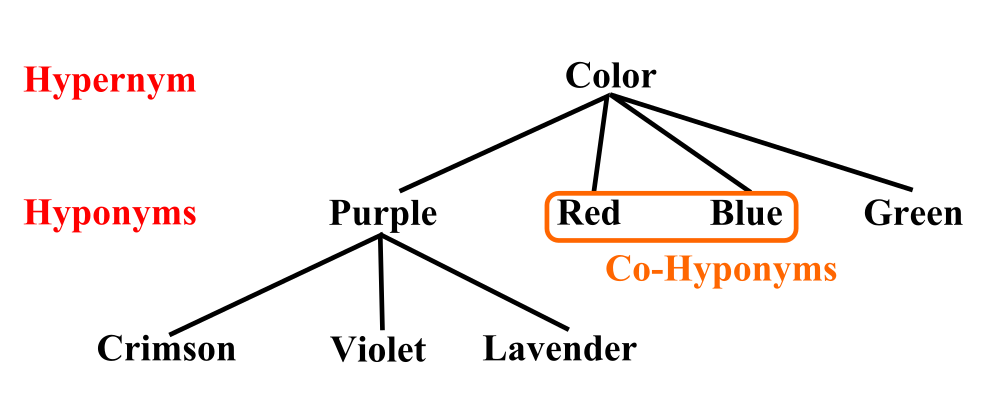
\includegraphics[width=\linewidth]{figs/hypernyms.png}
    \caption{An example of the hierarchy between hyponyms and hypernym [\url{https://en.wikipedia.org/wiki/Hyponymy_and_hypernymy}]}
    \label{fig:hypernyms}
\end{figure}

\begin{figure*}
    \centering
    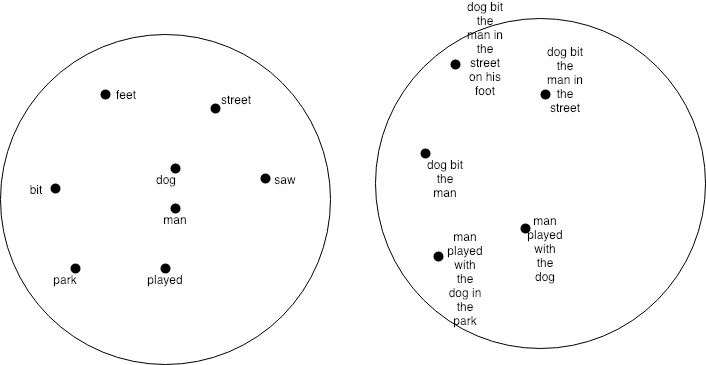
\includegraphics[width=\linewidth]{figs/semantic_hierrachy_captured.png}
    \caption{Semantic hierarchy captured in hyperbolic space}
    \label{fig:semantic_hierarchy}
\end{figure*}

\section{Related work}
In a short time there has been new and exciting work which aims to use the geometry of Hyperbolic Space to learn representations of natural language. ``\newcite{Nickel2017PoincarEF}'' train hyperbolic embeddings for WordNet ~\cite{Miller95wordnet} and test them for transitive closure and lexical entailment task. ``\newcite{dhingra2018embedding}'' focus on learning sentence embedding in an unsupervised manner using Skip-Thoughts \cite{skipthought} like framework. ``\newcite{hyperbolicqa}'' use hyperbolic representations of questions and answers to perform Question-Answering task on several different datasets. However, all these approaches use either a projection or reparameterization to convert representations in Euclidean Space to representations in Hyperbolic Space. Moreover, they use neural networks which are partially in Euclidean Space and partially in Hyperbolic Space. ``\newcite{poincareglove}'' successfully train hyperbolic word representations from scratch using a GloVe \cite{glove} like approach. Going a step further, ``\newcite{hyperbolicnn}'' train neural network with states as well as parameters in hyperbolic space to perform tasks like textual entailment and noisy prefix recognition. Continuing on the lines of these last two works, starting from training unsupervised hyperbolic embeddings and using hyperbolic neural network layers, we wish to propose and use hyperbolic attention mechanisms to perform the task of Natural Language Inference.


\section{Your approach}

As pointed out earlier, most of the previous approaches use hyperbolic space just for the intermediate representations by projecting or reparameterizing Euclidean Representations or word embeddings. This approach has proved partially successful. However, we believe that an end-to-end hyperbolic neural network based approach is more natural and might perform better. In our work, we would be starting by training our own word embeddings in the Hyperbolic Space (Poincar\'e ball model) in an unsupervised manner following the approach outlined in ``\newcite{poincareglove}''. Starting with these pretrained embeddings, we will use the hyperbolic analogs of standard recurrent neural networks (GRU or LSTM) ~\cite{hyperbolicnn} to perform the task of Natural Language Inference and compare it with a baseline formed by performing the same task using the Euclidean analog of our model. We will then move on to the main proposed contribution of this work -- propose and analyze different attention mechanisms in hyperbolic space to improve our model. 

Continuing on the work of ``\newcite{hyperbolicnn}'', which proposes hyperbolic analogs of linear (matrix multiplication in euclidean vector space) and non-linear transformations (pointwise non-linearity), we will use the operations in gyrovector space \cite{ungar2005} to come up with the formulation of different attention mechanisms in the Hyperbolic Space. We will compare the performance of these attention mechanisms with the baseline Euclidean attention analogs, on the task of Natural Language Inference.

\subsection{Expected Challenges}

We expect several challenges with the approach proposed above. Firstly, all the current deep learning frameworks are designed to work with parameters in Euclidean Space. Hence, we will not be able to use the gradients computed by these frameworks directly during optimization. However, as pointed out in ``\newcite{hyperbolicnn}'', one can transform the Euclidean Gradient to Hyperbolic Gradient. Secondly, due to the presence of transcendental functions in the formulas for operations in Poincar\'e Ball model of the Hyperbolic Space, we might face issues with numerical stability and convergence during optimization. In that scenario, we will try to mitigate the issue by performing suitable initialization of the model parameters. 


\subsection{Milestones \& Schedule}
We plan to write progress report and the final report as we work on the models. 
\begin{enumerate}
    \item Prepare the baseline model (responsibility? time?)
    \item Prepare hyperbolic word embeddings (responsibility? time?)
    \item Implement layers of the hyperbolic NN (responsibility? time?)
    \item Implement hyperbolic attentions (responsibility? time?)
    \item Write progress report! (Responsibility? due Apr 1)
    \item Analyze the performance of hyperbolic attention compared to the baseline, try different initializations and hyperparameters. If it works, why? If it doesn't then why? (Responsibility? time?)
    \item Work on final report and presentation (All. Time?)
\end{enumerate}


\section{Data}


We will evaluate the Hyperbolic Neural Networks with Attention mechanism over  Multi-Genre Natural Language Inference (MultiNLI) corpus. The dataset is designed to evaluate the machine learning models in how well they understand the sentence. the dataset is comprehensive with 443K samples of hypothesis/premise pairs and exhaustive in its coverage as it contains data from ten different genres of English language (written and spoken) which ensures that it covers the language in almost all its complexity.
The data is readily available from the website \url{https://www.nyu.edu/projects/bowman/multinli/}.
For model evaluation we will make use of held out data in the MultiNLI competition hosted on Kaggle \url{https://www.kaggle.com/c/multinli-matched-open-evaluation/data}.
The sentence pairs in the data is already annotated with textual entailment information so no further text annotation is required. The MultiNLI dataset fits the current scenario as the proposed Hyperbolic Neural Networks with Attention Mechanism allows us to explore the spectrum of Natural language Understanding in the hyperbolic space same as the dataset which has been proven to be a benchmark dataset in the field of Natural Language Understanding.\newcite{Williams2018ABC}.
is one of t he various tasks we plan to do with the Hyperbolic Neural Networks with Attention mechanism. For Language Modeling we will be using the 1Billion 


\section{Tools}

For this project we will predominantly be using PyTorch and Gensim.
PyTorch is a Python-based scientific computing package that is quickly growing as deep learning research platform that allows its users to harness the power of GPU. Gensim is a vector space modeling toolkit we will use to pretrain hyperbolic word embeddings using the approach mentioned in \newcite{poincareglove}. This project requires basic data processing and for training Language Model(if time permits) the data will be used in its crude form. We will be implementing Deep learning libraries by writing them from the scratch and implementing analog of basic blocks of Neural Networks like Feed Forward Layer, Non Linear activations and Attention Layer in the hyperbolic space. In order to do the compute we plan to use the Google Colab GPUs assuming they will allow the modularities within the model to run parallely else we will opt to run the model (training) on AWS or Microsoft Azure. The datasets we plan to use for the project is readily available so we don't need crowdsourcing.


\bibliographystyle{apalike}
\footnotesize
\bibliography{yourbib,attention}


\end{document}
